
\documentclass[]{svmono}

\usepackage{fancybox}
\usepackage{graphicx}
\usepackage{pdfpages}
\usepackage{color}
\usepackage{epstopdf}
\usepackage{geometry}
\usepackage{amsmath}
\usepackage{float}
\usepackage{listings}
\usepackage{verbatim}
\usepackage{booktabs}
\usepackage{tabularx}
\usepackage{longtable}
\usepackage{amsmath}
\usepackage{caption}
\usepackage{wrapfig}

\geometry{
 a4paper,
 total={210mm,297mm},
 left=20mm,
 right=20mm,
 top=20mm,
 bottom=15mm,
 }


\usepackage{subcaption}


\usepackage{enumerate}

\usepackage{bashful}

\usepackage{multicol}


\usepackage{textcomp}
\usepackage{hyperref}
%\usepackage[hyphenbreaks]{breakurl}
%\usepackage[hyphens]{url}


\sloppy
\definecolor{lightgray}{gray}{0.5}
\setlength{\parindent}{20pt}


\definecolor{mygreen}{rgb}{0,0.6,0}
\definecolor{mygray}{rgb}{0.5,0.5,0.5}
\definecolor{mymauve}{rgb}{0.58,0,0.82}

\lstset{ %
  backgroundcolor=\color{white},   % choose the background color; you must add \usepackage{color} or \usepackage{xcolor}
  basicstyle=\footnotesize,        % the size of the fonts that are used for the code
  breakatwhitespace=false,         % sets if automatic breaks should only happen at whitespace
  breaklines=true,                 % sets automatic line breaking
  captionpos=b,                    % sets the caption-position to bottom
  commentstyle=\color{mygreen},    % comment style
  deletekeywords={...},            % if you want to delete keywords from the given language
  escapeinside={\%*}{*)},          % if you want to add LaTeX within your code
  extendedchars=true,              % lets you use non-ASCII characters; for 8-bits encodings only, does not work with UTF-8
  frame=single,                    % adds a frame around the code
  keepspaces=true,                 % keeps spaces in text, useful for keeping indentation of code (possibly needs columns=flexible)
  keywordstyle=\color{blue},       % keyword style
  language=Python,                 % the language of the code
  morekeywords={*,...},            % if you want to add more keywords to the set
  numbers=left,                    % where to put the line-numbers; possible values are (none, left, right)
  numbersep=5pt,                   % how far the line-numbers are from the code
  numberstyle=\tiny\color{mygray}, % the style that is used for the line-numbers
  rulecolor=\color{black},         % if not set, the frame-color may be changed on line-breaks within not-black text (e.g. comments (green here))
  showspaces=false,                % show spaces everywhere adding particular underscores; it overrides 'showstringspaces'
  showstringspaces=false,          % underline spaces within strings only
  showtabs=false,                  % show tabs within strings adding particular underscores
  stepnumber=2,                    % the step between two line-numbers. If it's 1, each line will be numbered
  stringstyle=\color{mymauve},     % string literal style
  tabsize=2,                       % sets default tabsize to 2 spaces
  title=\lstname                   % show the filename of files included with \lstinputlisting; also try caption instead of title
}



\setlength{\parindent}{10pt}


\begin{document}




\begin{titlepage}    
\begin{center}
\vspace*{0in}
\huge{\sc  Old Dominion Univeristy\\  }



\vspace{1in}
\Large{\sc CS 495: Introduction to Web Science \\ Instructor: Michael L. Nelson, Ph.D \\ Fall 2014 4:20pm - 7:10pm R, ECSB 2120\\}

\vspace{1in}
\Large{Assignment \# 9\\}

\vspace{.5cm}
\Large{ \sc George C.  Micros  UIN: 00757376\\ }



\vspace {7cm}

{\large \bf {Honor Pledge}}\\
{I pledge to support the Honor System of Old Dominion University. I will refrain from any form of academic dishonesty or deception, such as cheating or plagIiarism. I am aware that as a member of the academic community it is my responsibility to turn in all suspected violations of the Honor Code. I will report to a hearing if summoned. }\\
\vspace {.5cm}

{Signed \_\_\_\_\_\_\_\_\_\_\_\_\_\_\_\_\_\_\_\_\_\_\_\_\_\_\_\_\_\_\_\_\_\_}


\today
\end{center}
\end{titlepage}



%%%%%%%%%%%%%%%%%%%%%%%%%%%%%%%%%%%%%%%%%%%%%%%%%%%%%%%%%%%
\author{George C. Micros}
\title{Written Assignment 9}
\subtitle{Fall 2014 \newline  CS 495: Introduction to Web Science\newline Dr. Michael Nelson}
\maketitle

%%%%%%%%%%%%%%%%%%%%%%%%%%%%%%%%%%%%%%%%%%%%%%%%%%%%%%%%%%%

\tableofcontents

\chapter{Written Assignment 9}

\noindent



\section{Question 1}

\subsection{The Question}

\begin{flushleft}

What 5 movies have the highest average ratings? Show the movies
and their ratings sorted by their average ratings.

\end{flushleft}
\subsection{The Answer}


\begin{flushleft}
\begin{table}[h]
\centering
\begin{tabular}{ll}

5.0000 & They Made Me a Criminal (1939)                          \\
5.0000 & Star Kid (1997)                                         \\
5.0000 & Someone Else's America (1995)                           \\
5.0000 & Santa with Muscles (1996)                               \\
5.0000 & Saint of Fort Washington The (1993)                     \\
5.0000 & Prefontaine (1997)                                      \\
5.0000 & Marlene Dietrich: Shadow and Light (1996)               \\
5.0000 & Great Day in Harlem A (1994)                            \\
5.0000 & Entertaining Angels: The Dorothy Day Story (1996)       \\
5.0000 & Aiqing wansui (1994)                                    \\
4.6250 & Pather Panchali (1955)                                  \\
4.5000 & Some Mother's Son (1996)                                \\
4.5000 & Maya Lin: A Strong Clear Vision (1994)                  \\
4.5000 & Everest (1998)                                          \\
4.5000 & Anna (1996)                                             \\ \hline
4.4911 & Close Shave A (1995)                                    \\ \hline
4.4664 & Schindler's List (1993)                                 \\ \hline
4.4661 & Wrong Trousers The (1993)                               \\ \hline
4.4568 & Casablanca (1942)                                       \\
\end{tabular}
\caption{Highest Average Rating}
\end{table}

\end{flushleft}





%\section{Question 2}

\subsection{The Question}

\begin{flushleft}

What 5 movies received the most ratings? Show the movies and
the number of ratings sorted by number of ratings.

\end{flushleft}
\subsection{The Answer}

There review infromation is read in and appeneded to each movie. There is a counter that counter the number of reviews for each movie. This could also be determined by checking the length of the review list for each movie. 


\begin{lstlisting}[caption={Python code for question 2}]

def q2(movies):
	clearScore(movies)
	for i in reviews:
		movies[i.item-1].scores.append(float(i.score))
		movies[i.item-1].cnt +=1

	for i in movies:
		i.avgr();

	# MOST RATING
	mRate = sorted(movies, key=lambda x:x.cnt, reverse=True)
	f = open("q2.txt", "w")
	print "\n\tQ2: Most Ratings"
	for i in range(0,5):
		print  mRate[i].cnt, mRate[i].title
		f.write("% d,  \"%s\"\n" % (mRate[i].cnt, mRate[i].title))
	f.close()

\end{lstlisting}

\begin{flushleft}

\begin{table}[h]
\centering
\setlength{\tabcolsep}{12pt}
\begin{tabular}{|ll|}

\hline
583 & Star Wars (1977)          \\ \hline
509 & Contact (1997)            \\ \hline
508 & Fargo (1996)              \\ \hline
507 & Return of the Jedi (1983) \\ \hline
485 & Liar Liar (1997)         \\ \hline
\end{tabular}
\caption{Movies with Most Ratings}
\end{table}
\end{flushleft}





\section{Question 3}

\subsection{The Question}



 Consider the "bow-tie" graph in the Broder et al. paper (fig 9):
    \url{http://www9.org/w9cdrom/160/160.html}

    Now consider the following graph:

\begin{multicols}{4}


    A $ \rightarrow $ B

    B $ \rightarrow $ C

    C $ \rightarrow $  D

    C $ \rightarrow $ A

\columnbreak

    C $ \rightarrow $  G

    E  $ \rightarrow $  F

    G $ \rightarrow $ C

    G $ \rightarrow $ H

    I $ \rightarrow $ H

\columnbreak

    I $ \rightarrow $ J

    I $ \rightarrow $ K

    J $ \rightarrow $ D 

    L $ \rightarrow $ D

\columnbreak

    M $ \rightarrow $ A

    M $ \rightarrow $ N

    N $ \rightarrow $ D
    
\end{multicols}




    For the above graph, give the values for:  IN,   SCC,    OUT,  Tendrils,     Tubes,     Disconnected

\subsection{The Answer}


The most critical part of analyzing a graph and identifying the constituent components is to find the strongly connected component. This can be done visually or heuristically in this case. However, in the case of complex and large networks this is not an efficient method. Thankfully algorithms have been developed to solve this problem and they are implemented in python libraries. This way we can verify the result we obtain manually. 




\begin{figure}
\centering
	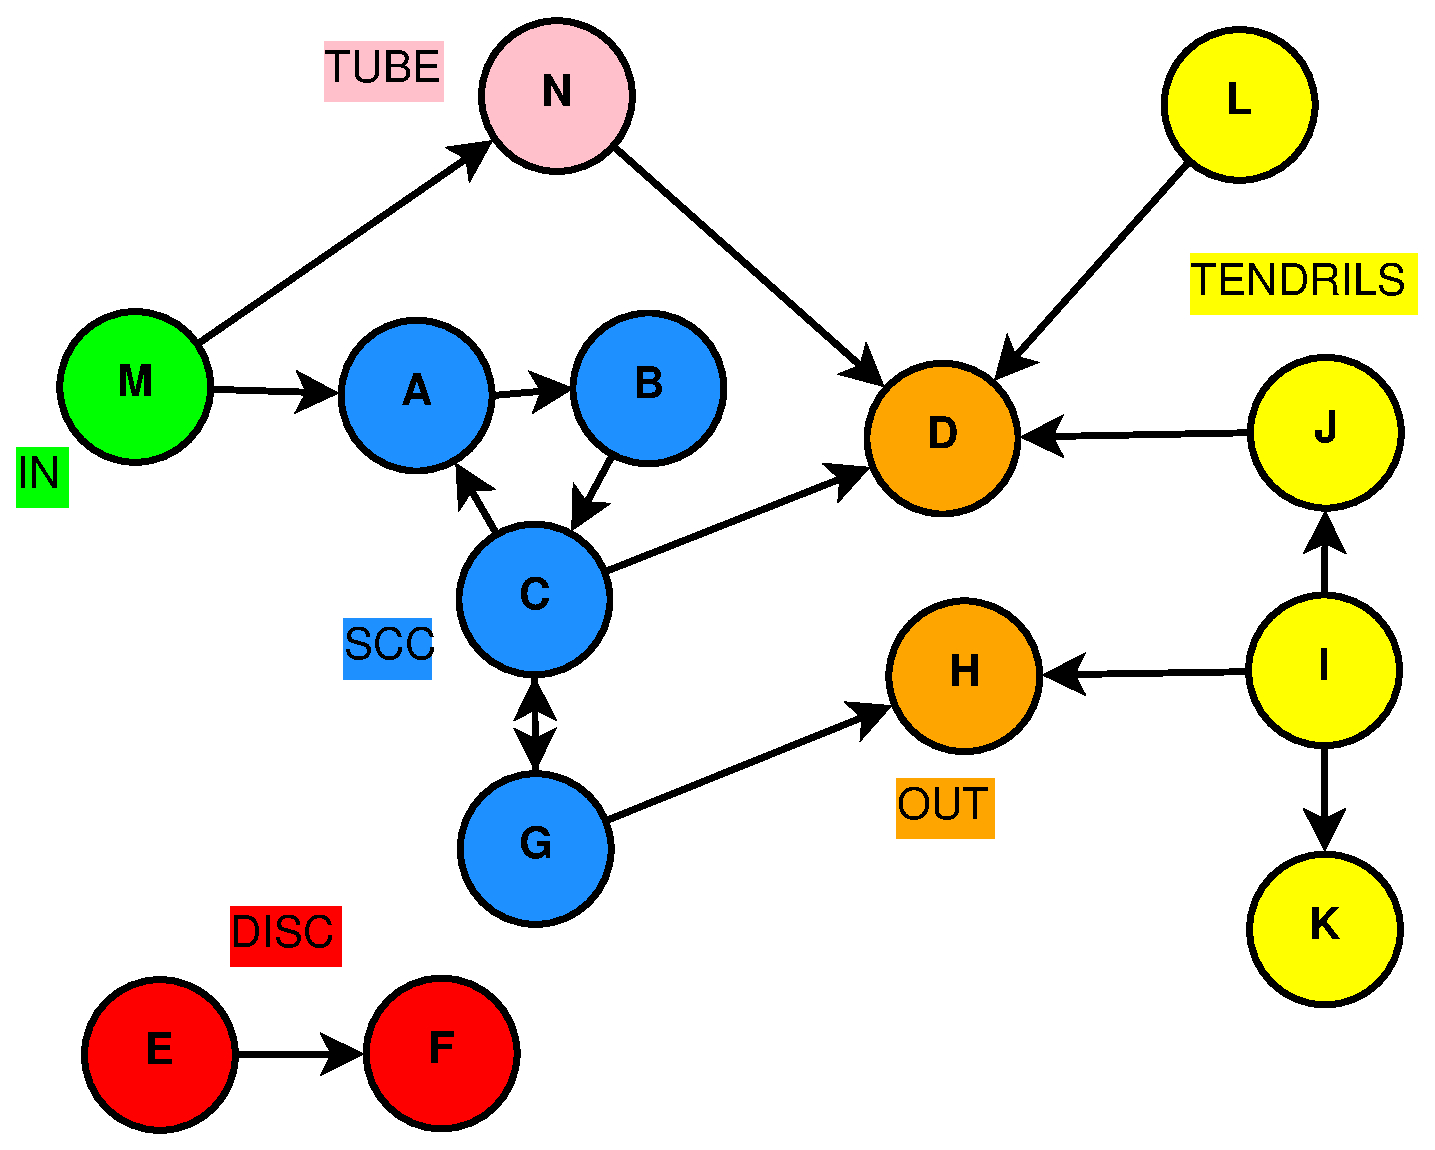
\includegraphics[width=.8\textwidth]{figures/graphLabel.eps}
	
\end{figure}


\pagebreak

\lstset{
    language=python,
    label=code:correction_8.5,
    caption={Code Listing the relevance file corrector}
}

\lstinputlisting{../q3/graphSc.py}
\section{Question 3}

\subsection{The Question}

\begin{flushleft}

 Cluster the blogs using K-Means, using k=5,10,20. (see slide 18).
How many interations were required for each value of k?

\end{flushleft}
\subsection{The Answer}

The Python function used to produce the K-Means is provided in the book \cite{PCI}. Clustering into 5 clusters required 7 iterations. Clustering into 10 clusters required 6 iterations. Clustering into 20 clusters required 6 iterations.  The terminal output for the script is provided and displays that cluster members


\lstset{
    language=Python,
    label=code:q1,
    caption={Python script to produce dendrograms}
}
\lstinputlisting{../q3/q3.py}


\begin{figure}
\centering
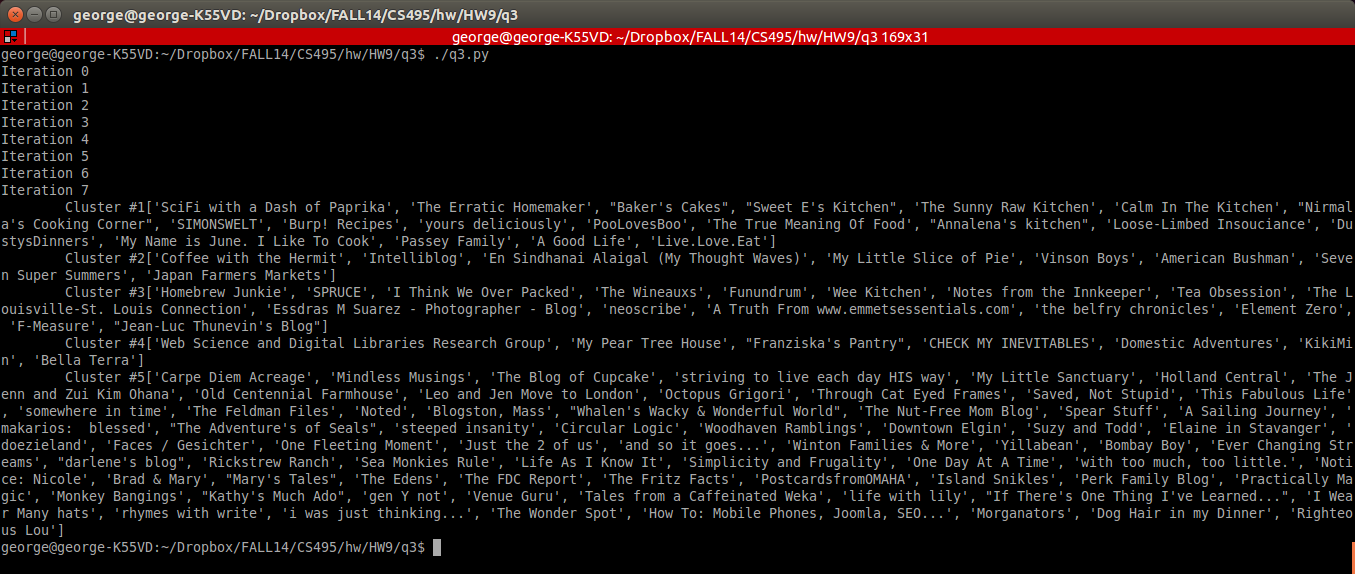
\includegraphics[width=\textwidth]{../q3/clust5.png}
\caption{Terminal output from K-Means CLustering, k = 5}
\end{figure}


\begin{figure}
\centering
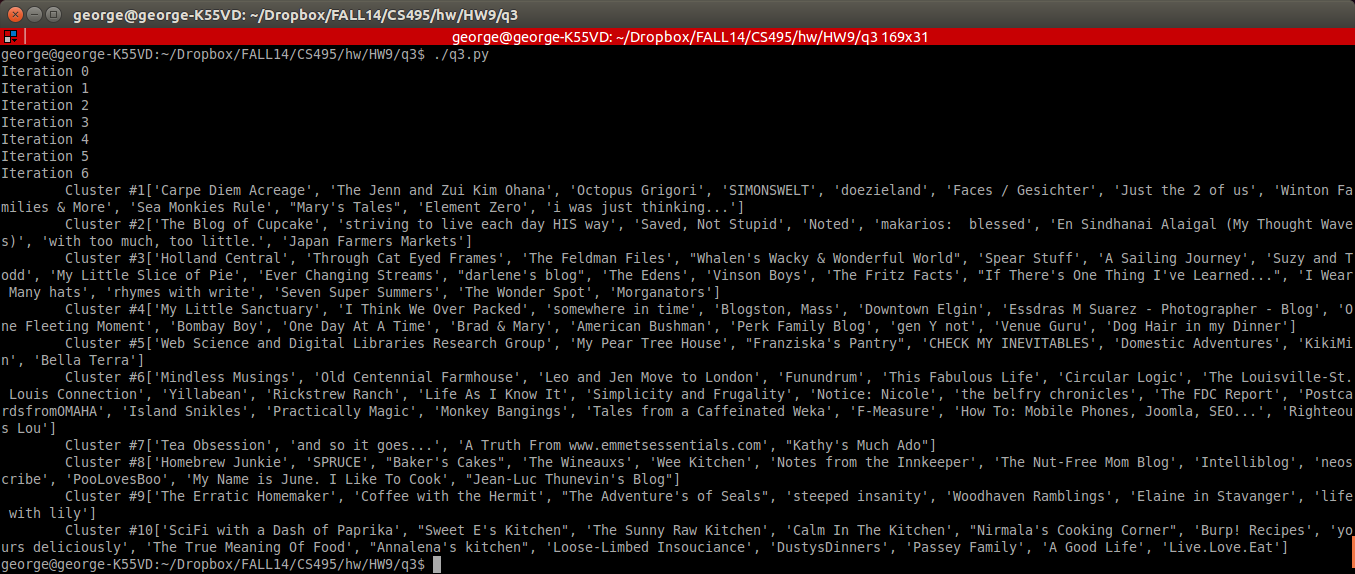
\includegraphics[width=\textwidth]{../q3/clust10.png}
\caption{Terminal output from K-Means CLustering, k = 10}
\end{figure}

\begin{figure}
\centering
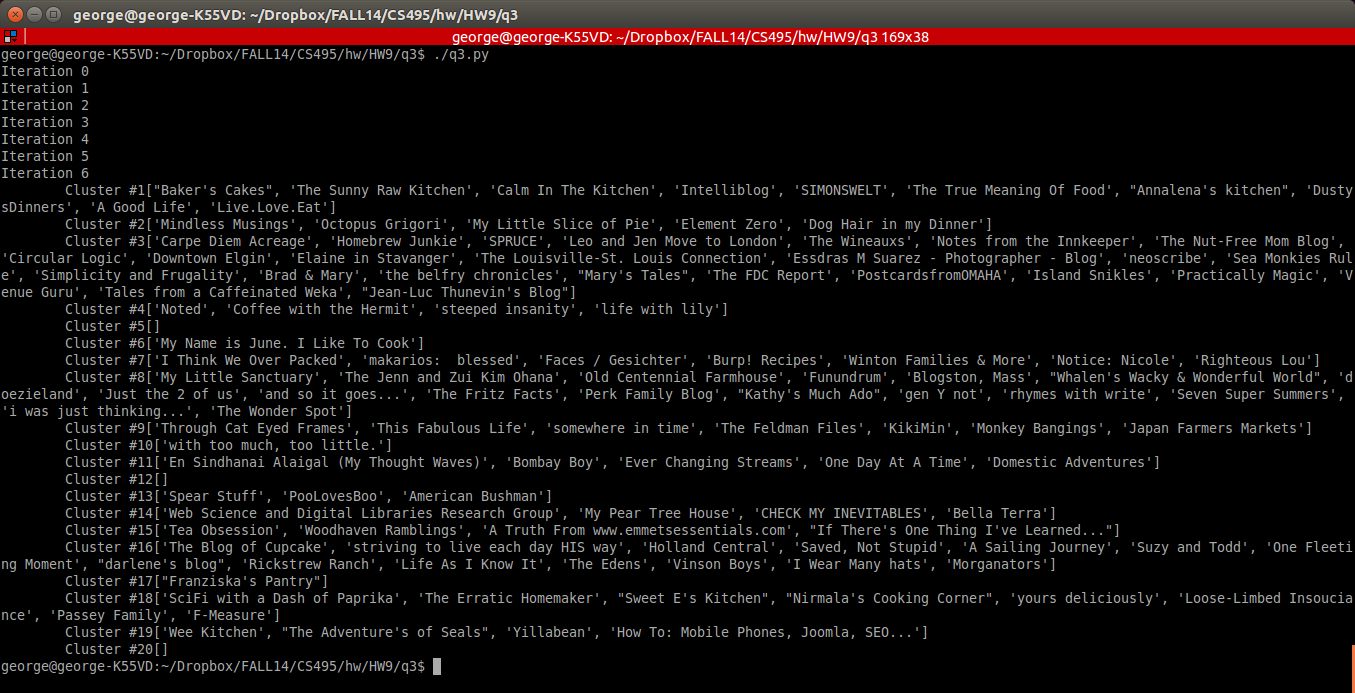
\includegraphics[width=\textwidth]{../q3/clust20.png}
\caption{Terminal output from K-Means CLustering, k = 20}
\end{figure}




\section{Question 4}

\subsection{The Question}

\begin{flushleft}

 Use MDS to create a JPEG of the blogs similar to slide 29.  
How many iterations were required?

\end{flushleft}
\subsection{The Answer}


The Python function used to produce the MDS plot is provided in the book \cite{PCI}. The algorithm required 353 iterations to converge. The terminal output it attached.

\lstset{
    language=Python,
    label=code:q1,
    caption={Python script to produce dendrograms}
}
\lstinputlisting{../q4/q4.py}


\begin{figure}
\centering
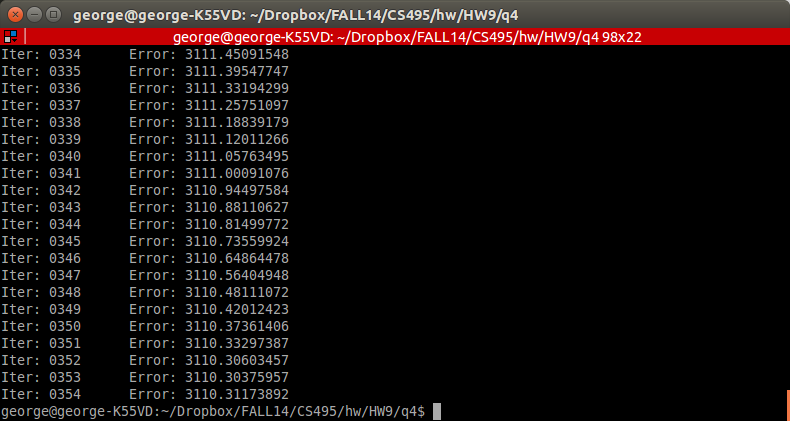
\includegraphics[width=\textwidth]{../q4/mds.png}
\caption{Terminal output from Multi-Dimensional Scaling}
\end{figure}

\begin{figure}
\centering
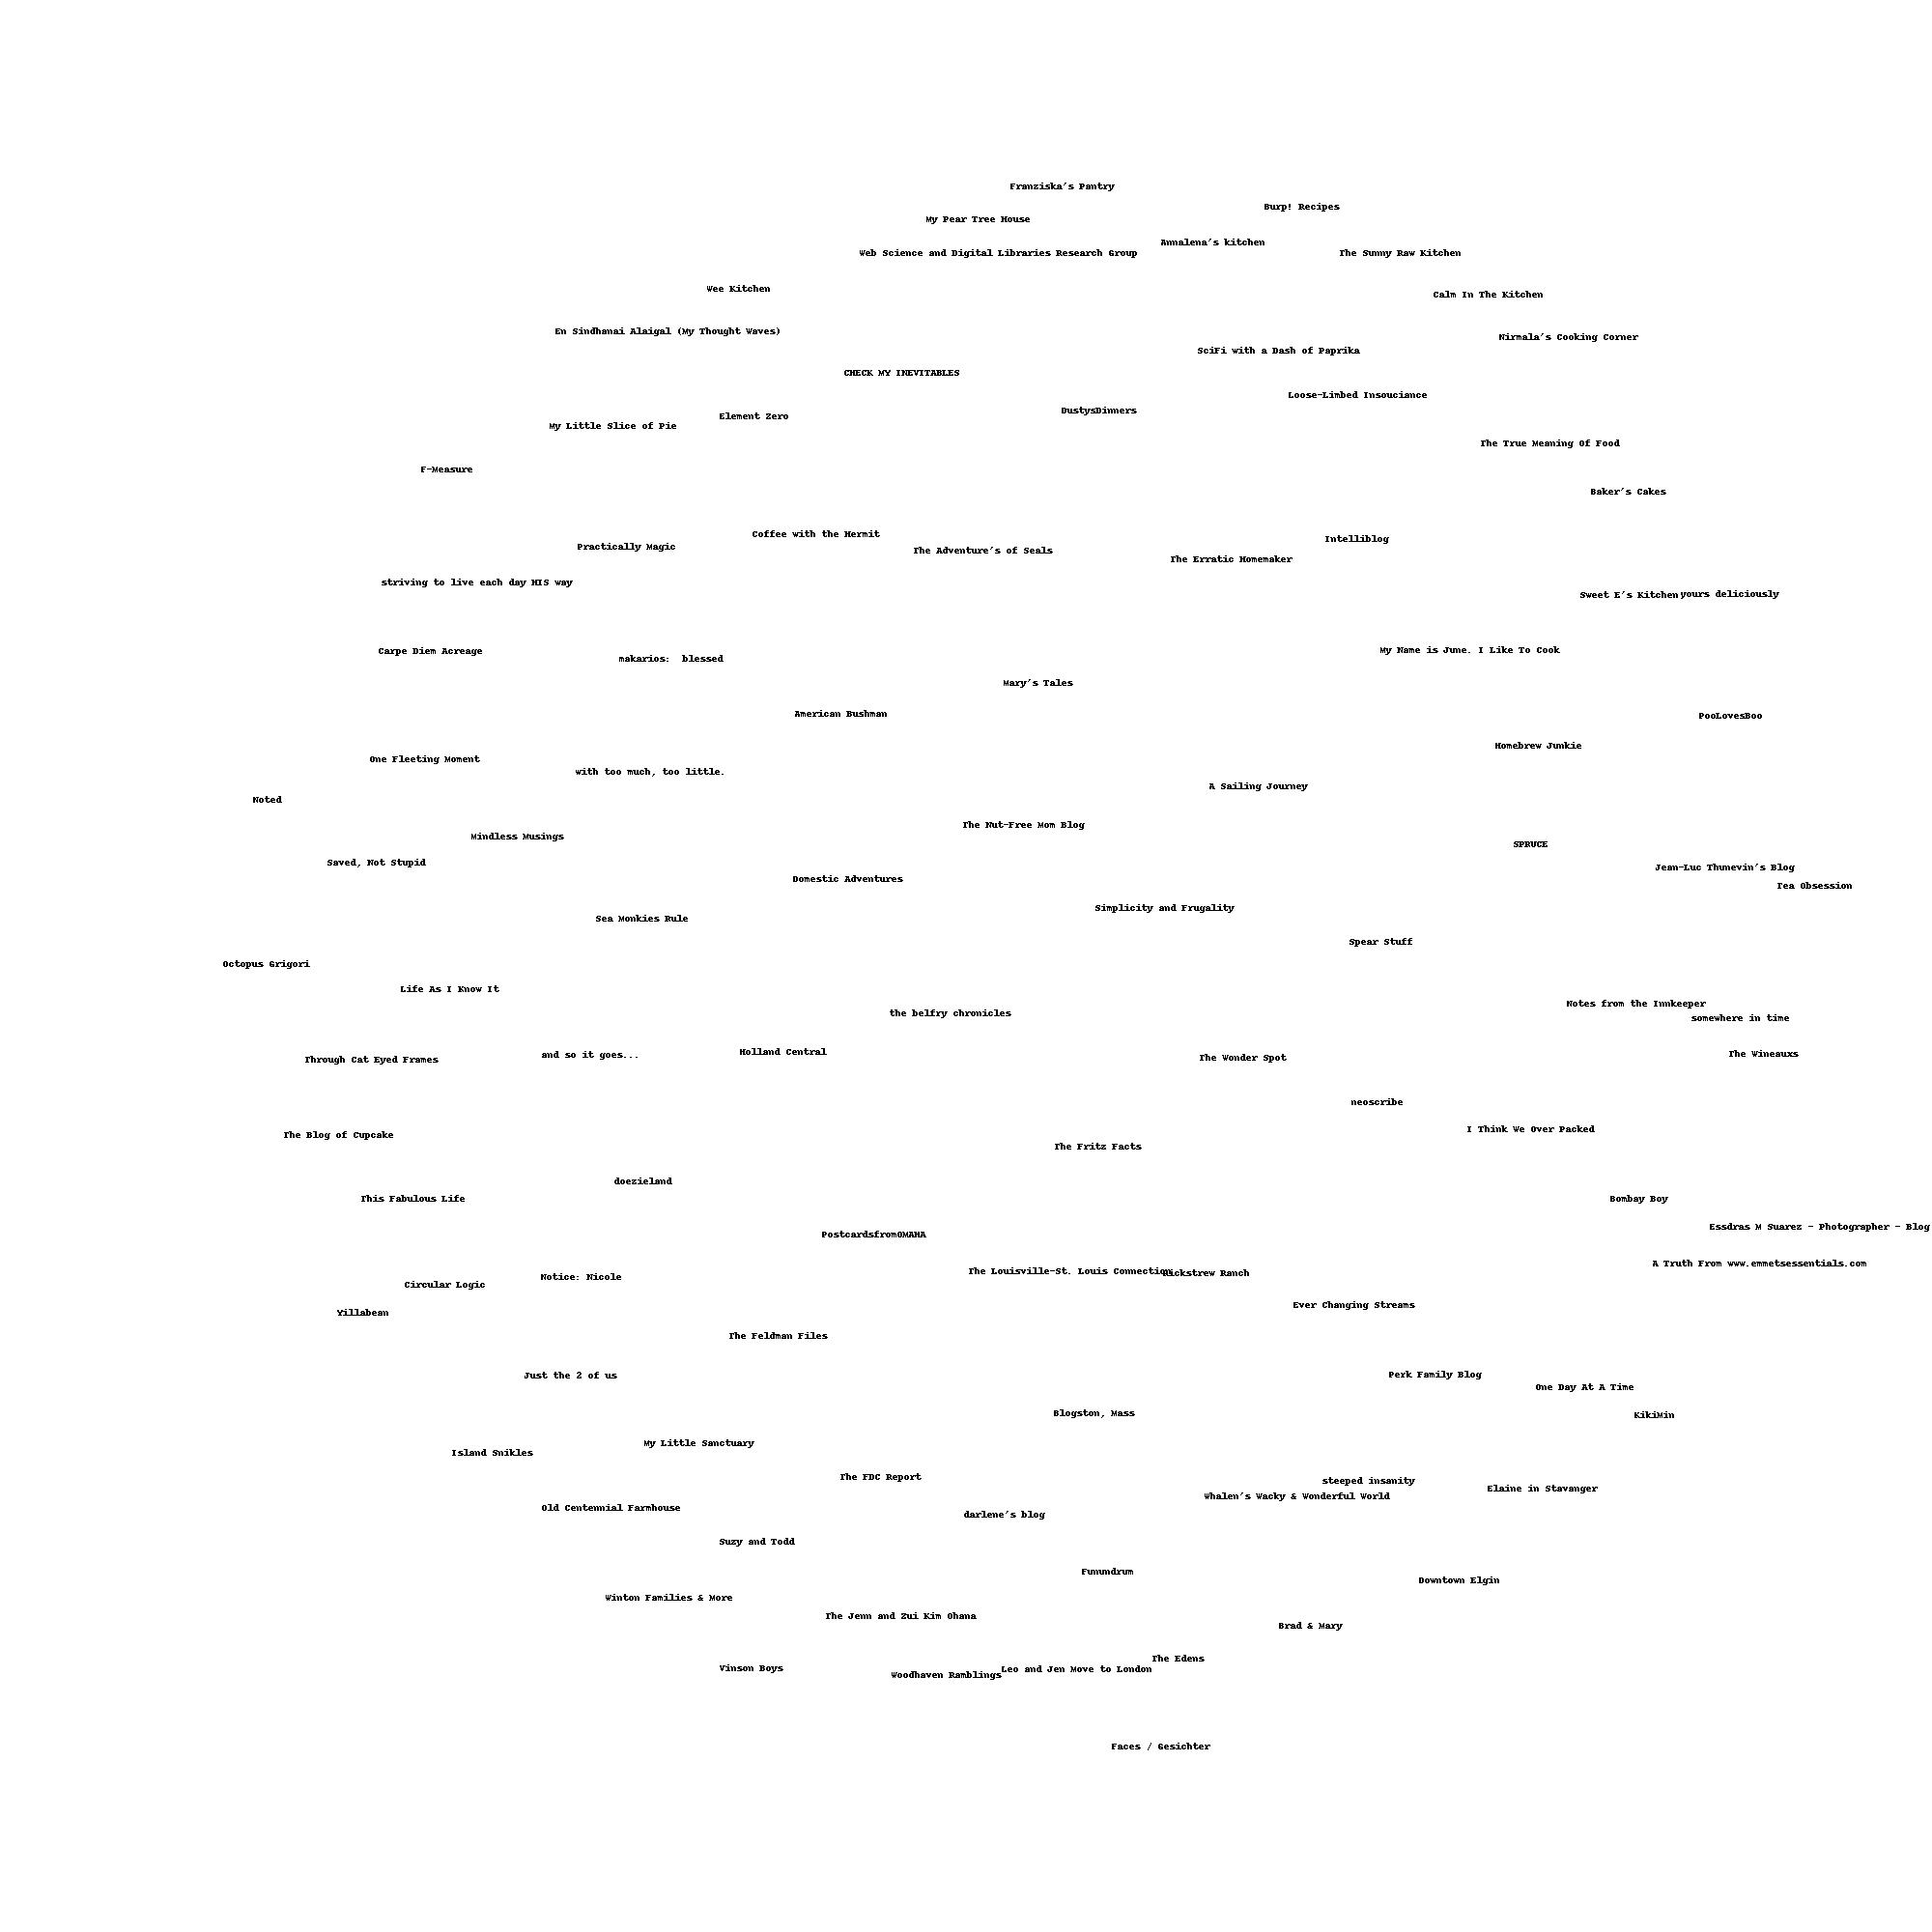
\includegraphics[width=\textwidth]{../q4/blogs2d}
\caption{Multi-Dimensional Scaling of the blogs}
\end{figure}





\section{Extra Credit Question}

\subsection{The Question}

\begin{flushleft}

Re-run question 2, but this time with proper TFIDF calculations
instead of the hack discussed on slide 7 (p. 32).  Use the same 500
words, but this time replace their frequency count with TFIDF scores
as computed in assignment \#3.  Document the code, techniques,
methods, etc. used to generate these TFIDF values.  Upload the new
data file to github.

Compare and contrast the resulting dendrogram with the dendrogram
from question \#2.

Note: ideally you would not reuse the same 500 terms and instead
come up with TFIDF scores for all the terms and then choose the top
500 from that list, but I'm trying to limit the amount of work
necessary.

\end{flushleft}
\subsection{The Answer}


The TFIDF calculation requires the computation of two numbers, the term frequency and the inverse document frequency.
The {\sl term frequency} (TF) is defined as the frequency of the term in the document normalized by the number of terms in the document. 

\begin{center}
\Large
$TF = \frac{\text{number of term occurances}}{\text{number of words in document}}$
\end{center}

The {\sl inverse document frequency} (IDF) of the query is defined as the log base 2 of the number of webpages in the corpus over the number of webpages containing the term. 




\begin{center}
\Large
$IDF =\log_{2} (\frac{\text{number of webpages in corpus}}{\text{number of webpages containing the term}})$
\end{center}


	In the context of the blog matrix this can be visualized easily. Each row consists of a blog vector and each column consists of a term column vector. The elements of the matrix are the occurance frequency of a given term in a specific blog. The code essentially scaled the frequency by the lenght of the blog feed, but that is constant across all terms. The term frequency of a term in a blog is the frequency divided by the number of terms in the blog. In the matrix that is the element value divided by the length of the blog vector. Then summing across all blogs gives the sum of the term frequencies of all blogs which results in a vector of length equal to the number of terms in the corpus. This is the TF value. 	The numerator of the IDF value is constant across all terms and therefore irrelevant. The denominator is the number of blogs that the term appeared it. In matrix view, this represents the number of non-zero elements in a column.
Unfortunately the implementation the book used was not matrix based and therefore some magic had to take place to figure out how to compute these values. However the proper use of dictionaries made the implemention efficient and straight-forward.




\begin{lstlisting}
tf = {}
    blogs = wordcounts
    # go through every blog
    for blog in blogs:
        # go through every term
        for term in blogs[blog]:
            if term in tf: 
                tf[term] += blogs[blog][term]/float(len(blogs[blog])) 
            else:
                tf[term] = blogs[blog][term]/float(len(blogs[blog])) 
    corp = float(len(blogs))
    idf = {}
    for i in apcount:
        idf[i] = log(corp/apcount[i])/log(2)
    tfidf = {}
    for i in tf:
        tfidf[i] = tf[i]*idf[i]
    new = []
    for i in tfidf:
        new.append((i, tfidf[i]))
    new.sort(key=lambda tup:tup[1], reverse=True)
    wordlist = []
    for i in range(500):
        print new[i][0]
        wordlist.append(new[i][0].encode('ascii'))

\end{lstlisting}

The overall accuracy of the two methods is hard to evaluate in an absolute scence because the blogs are not labeled in a way that provides insight to an absolute form of clustering. An attempt to create clusters manually based on the content is not objective and can be easily mislead by our perception of the blogs. Therefore there is no method to score the outcome can then compare the score of the two techniques. 

The one things that does seem to stand out is the distinct tree structure that the two methods display. This become more clear when they are placed alongside each other. The naive term frequency tree seems to randomly split at every iteration. Groupings split up in unequal groups at each step, i.e. a cluster will split up into two clusters, one containing a single blog and then other the rest. This shows that the groups are not very consistent and at the next split the outliers branch off into their own group. This process continues as each cluster loses a blog at each iteration and gets smaller, without any indication of a dictinct seperation into two groups. For example, the food cluster should split up into the desert and the entree clusters, but in this case the food cluster sheds a blog at a time. 

The TFIDF dendrogram appears more structured and precise, very close to binary tree. Throughout the entire process the clusters are divided into subgroups. There are occurances of the random ``one-off'' blog, but that is predictable. Also, the number of terms used is only 500, which many not be large enough to provide a proper result.  The TFIDF method appear to find dominant characteristics of the cluster to patition on. While the naive method finds the most eccentric member and removes him. 

One a more abstract, and slightly ``hand-wavy'', interpretation blogs represent the people that write them. A population can be clusters into in a variety of ways, i.e. hobby, occupation, gender, age, but the clusters that provide the most information are the ones that partition the cluster into the subgroups that are bound by a characteristic. This type of clustering is equivalent to a useful demographic map, e.g. young male engineers, young female engineers, retired wood craftsman, etc. The group can be used to describe its members in a reasonable way. However, the population can be clustered based on who is a Harvard graduate that is also in an underground alt-rock band and not.  There is lots of detail about one group, but there members of the other group are not held together by any common traits.  Adolf Hitler and Edward Snowden would be in the same cluster and then the question become what do they have in common. 
\begin{figure*}[t!]
        \centering
        \begin{subfigure}{0.5\textwidth}
	\centering
	 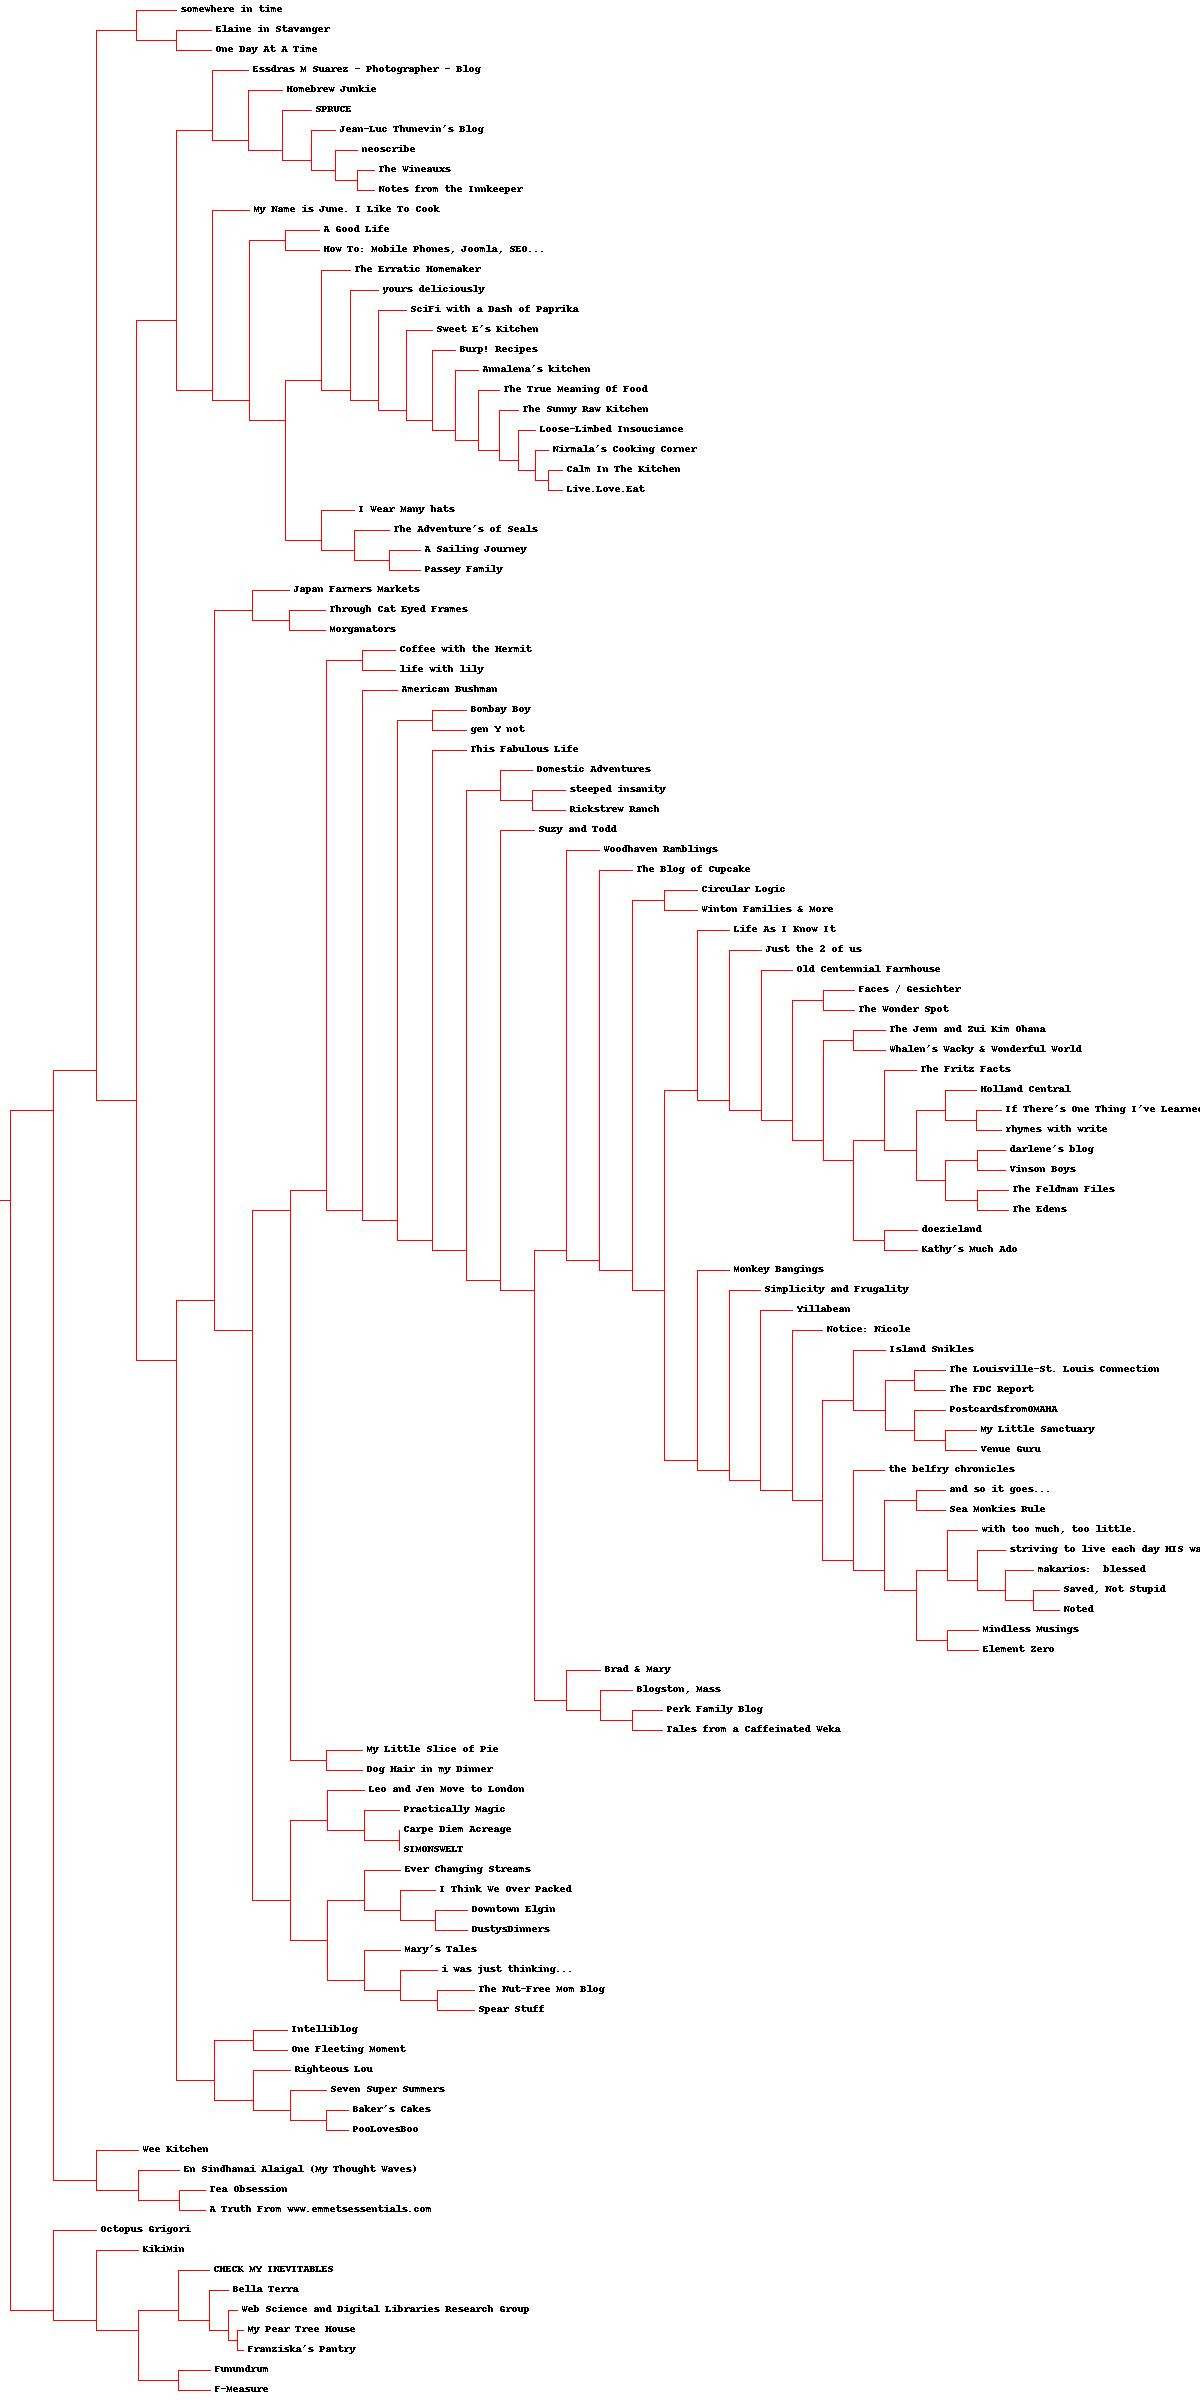
\includegraphics[height=11cm, width=9cm]{../q2/blogdendro.jpg}

             \caption{Dirty Hack}
        \end{subfigure}%
        \begin{subfigure}{0.5\textwidth}
		\centering
               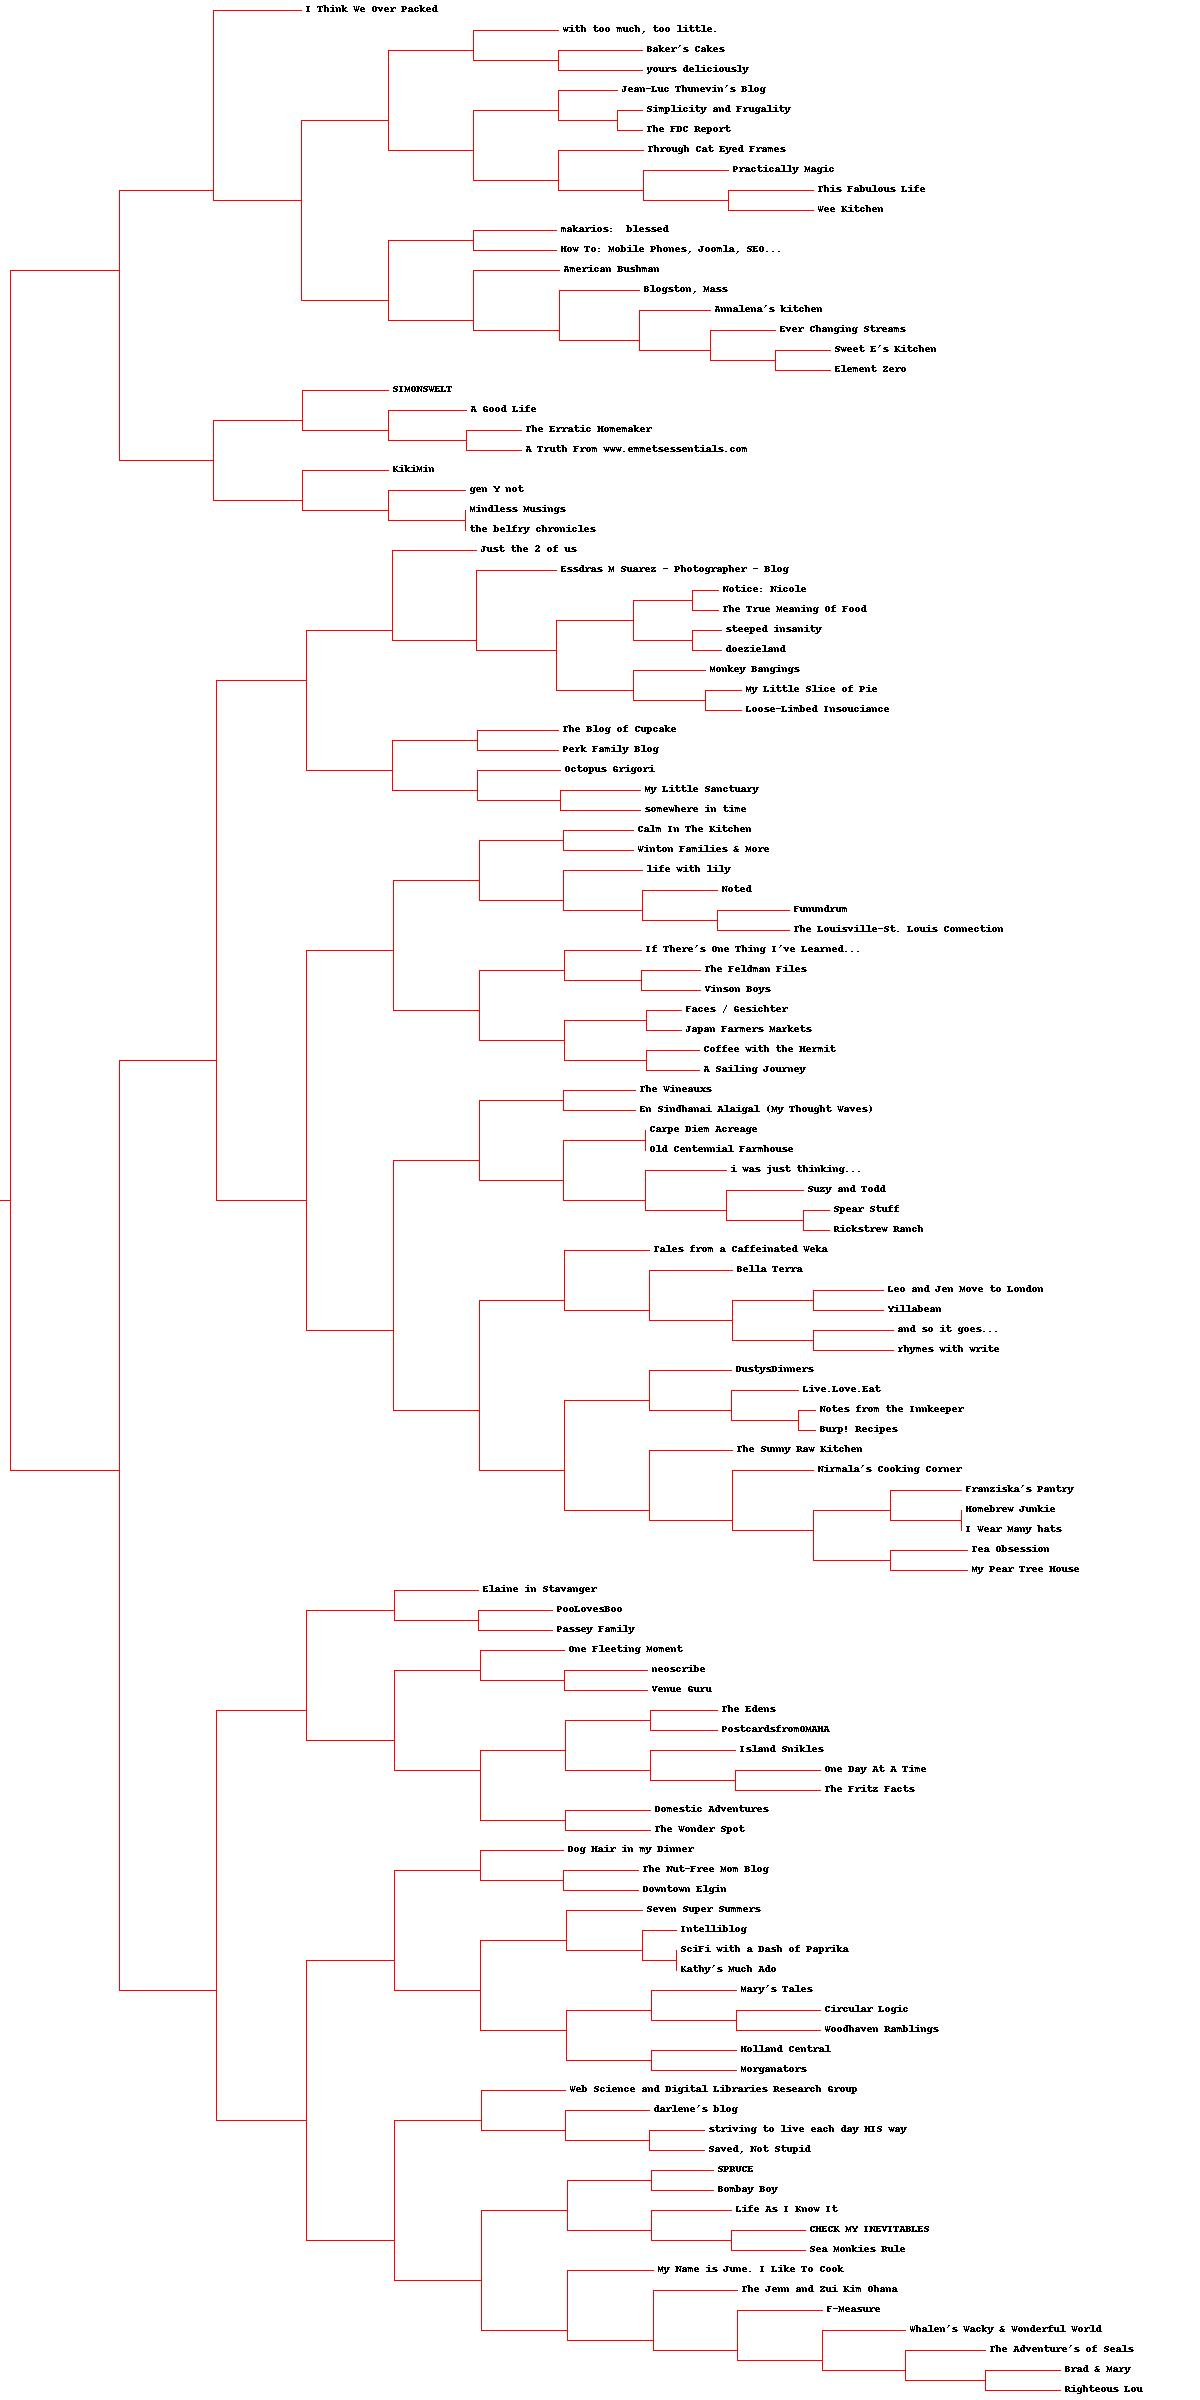
\includegraphics[height=11cm, width=9cm]{../qec/blogdendro}	
\caption{TFIDF}
        \end{subfigure}
    
\end{figure*}



In conclusion, my opinion is that the TFIDF measure clusters in a way that produces distinct subgroups which are meaningful and consistent. On the other hand, the naive approach partitions based on the odd one out, but sometime the odd one isnt very odd and the non-odd ones dont have much to do with each other. This is the conclusion that I draw based on the structure of the divisions. Even if the groups don't seem related based on the title they have some common characteristic that TFIDF can determine, but the naive method does not.








\begin{figure}[h!]
\centering
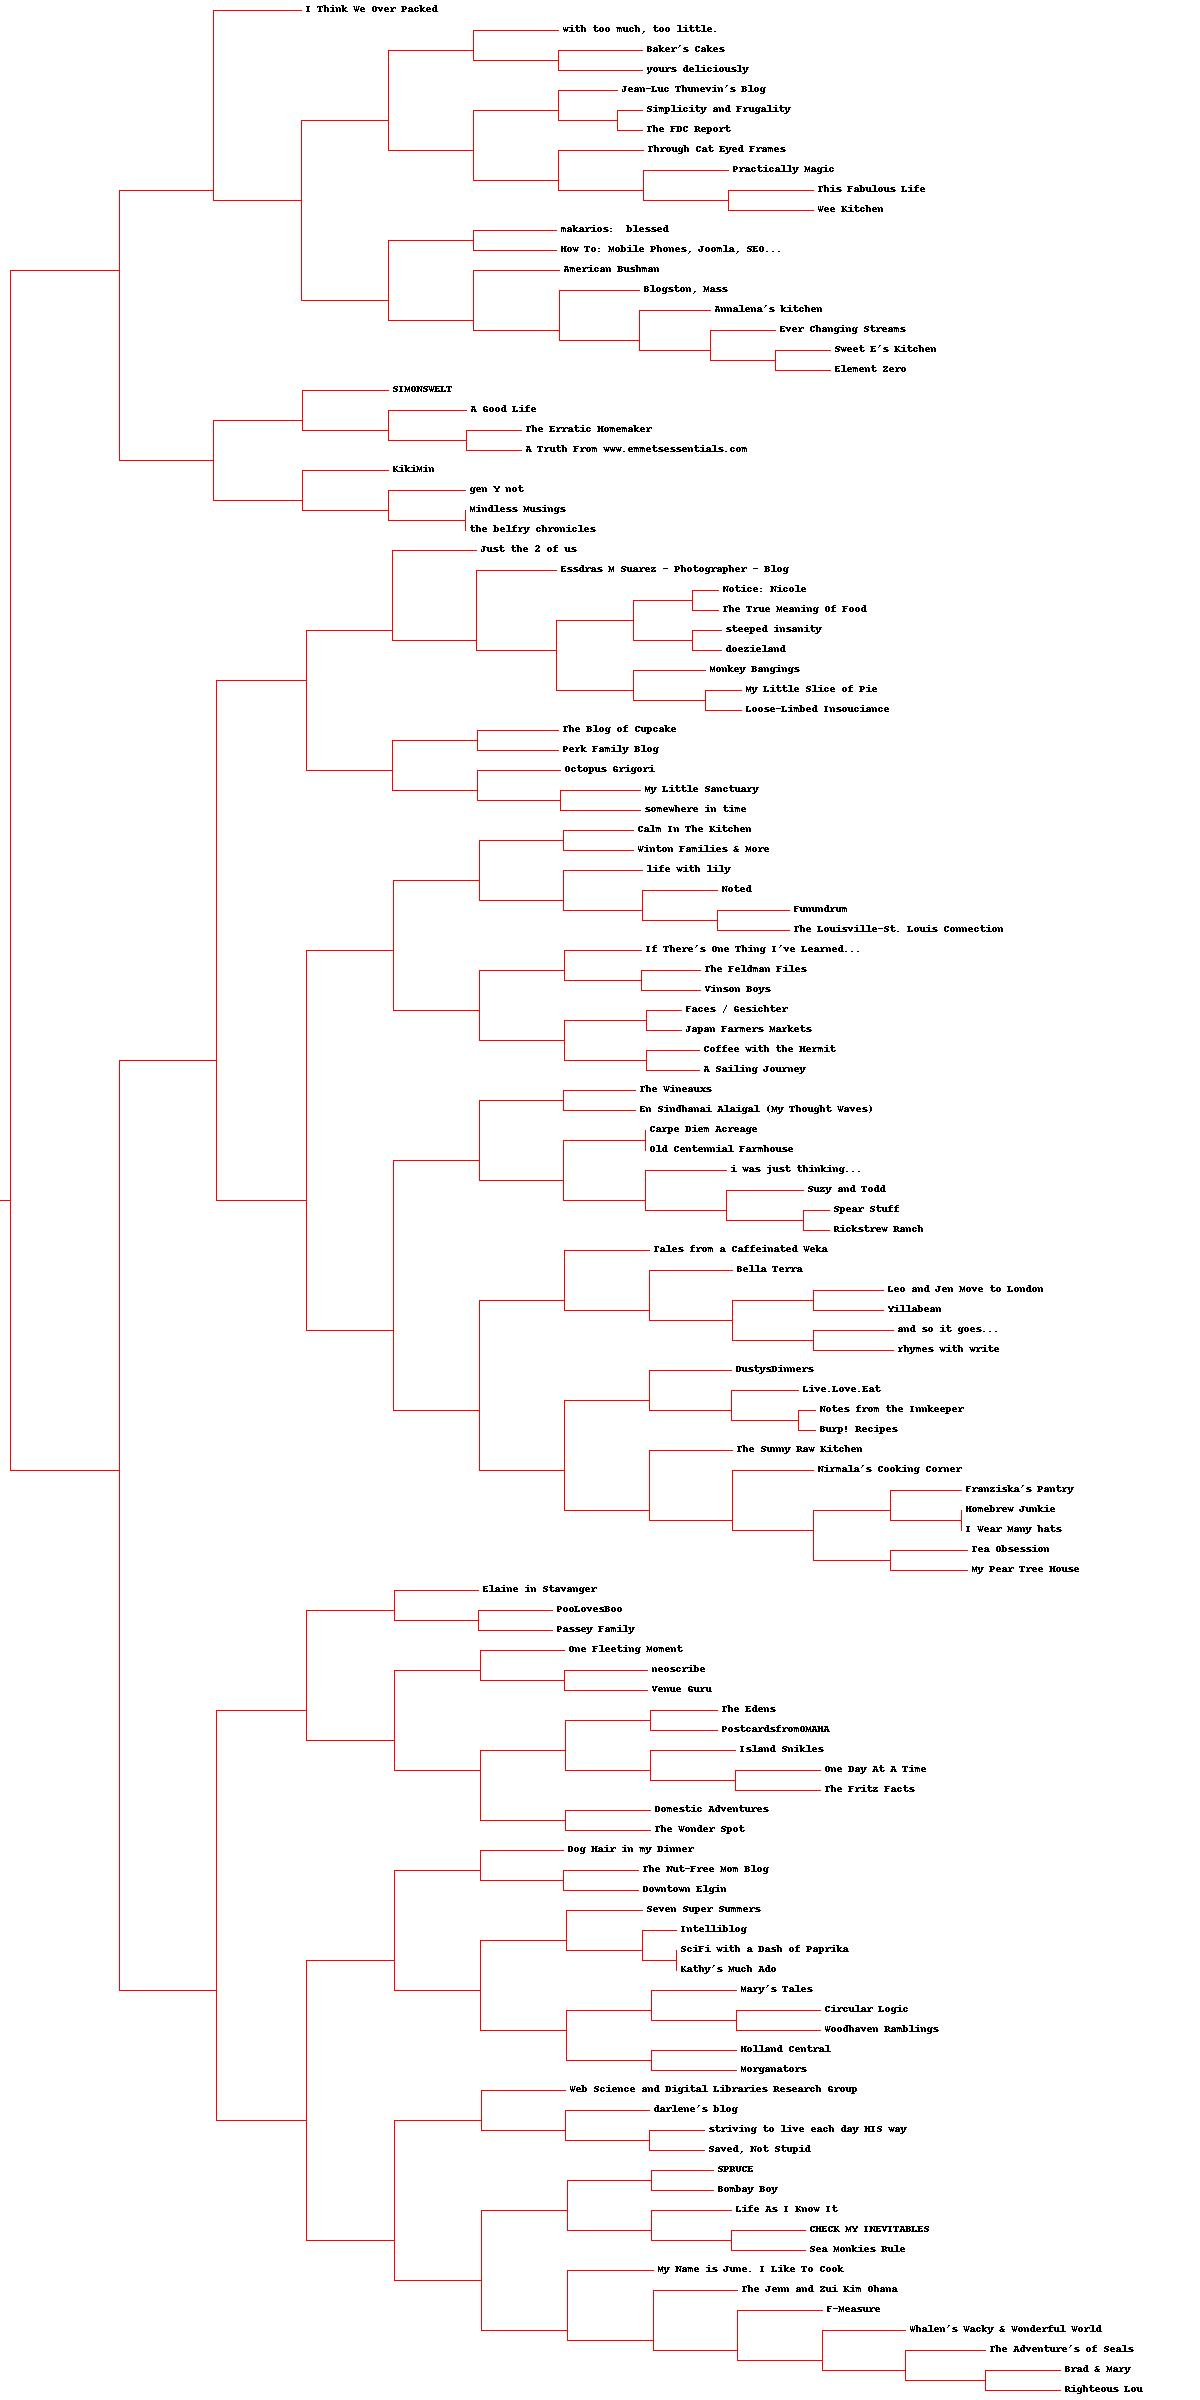
\includegraphics[height=25cm]{../qec/blogdendro}
\caption{TFIDF dendrogram}
\end{figure}







%%%%%%%%%%%%%%%%%%%%%%%%%%%%%%%%%%%%%%%%%%%%%%%%%%%%%%%%%%%


%%%%%%%%%%%%%%%%%%%%%%%%%%%%%%%%%%%%%%%%%%%%%%%%%%%%%%%%%%%
\nocite{*}
\bibliography{sources}
\bibliographystyle{unsrt}




%%%%%%%%%%%%%%%%%%%%%%%%%%%%%%%%%%%%%%%%%%%%%%%%%%%%%%%%%%%

%%%%%%%%%%%%%%%%%%%%%%%%%%%%%%%%%%%%%%%%%%%%%%%%%%%%%%%%%%%



%%%%%%%%%%%%%%%%%%%%%%%%%%%%%%%%%%%%%%%%%%%%%%%%%%%%%%%%%%%




%%%%%%%%%%%%%%%%%%%%%%%%%%%%%%%%%%%%%%%%%%%%%%%%%%%%%%%%%%%



%%%%%%%%%%%%%%%%%%%%%%%%%%%%%%%%%%%%%%%%%%%%%%%%%%%%%%%%%%%




\end{document}


